\documentclass[openany]{article} 
\usepackage[english]{babel}
\usepackage[utf8]{inputenc}
\usepackage[T1]{fontenc}
\usepackage{geometry} 
\usepackage{graphicx}
\usepackage{caption}
\usepackage{subcaption}

\title{Visual Data Analytics: Practical Exercise}
\date{WS 2022/2023}
\author{Matilde Tozzi}
%\renewcommand{\baselinestretch}{1.1}

\renewcommand{\thesubsection}{\thesection.\alph{subsection}}

\begin{document}

\maketitle

\section {First part: ParaView}

In the first section we use the ParaView software to test a wide range of visualisations.

\subsection {VisHuman Head}

For this task we used the \texttt{vmhead256cubed.raw} file. When opened in ParaView, we need to specify how the data is encoded in the file and this is done by setting the properties according to the \texttt{vmhead256cubed.dat} file, so in this case we had a dataset of 3D 0-255 values of \texttt{unsigned char} format. 

Then, we use a \textit{volume} rendering and we set the transfer function in order to display mostly the bones of the person, keeping the skin just in transparency. This is done by cutting the first peak of density values, that are mostly noise, and also the second peak of density values, that correspond to the majority of flesh. The highest density values, corresponding to the bones, are set to the maximum opacity. We used a modified version of the \textit{X Ray} color map.

\begin{figure}[h]
\centering
\begin{subfigure}{.45\textwidth}
  \centering
  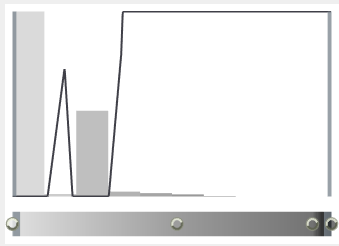
\includegraphics[width=\linewidth]{VisHuman_Head/transfer_function_1}
  \caption{Used transfer function}
\end{subfigure}%
\begin{subfigure}{.5\textwidth}
  \centering
  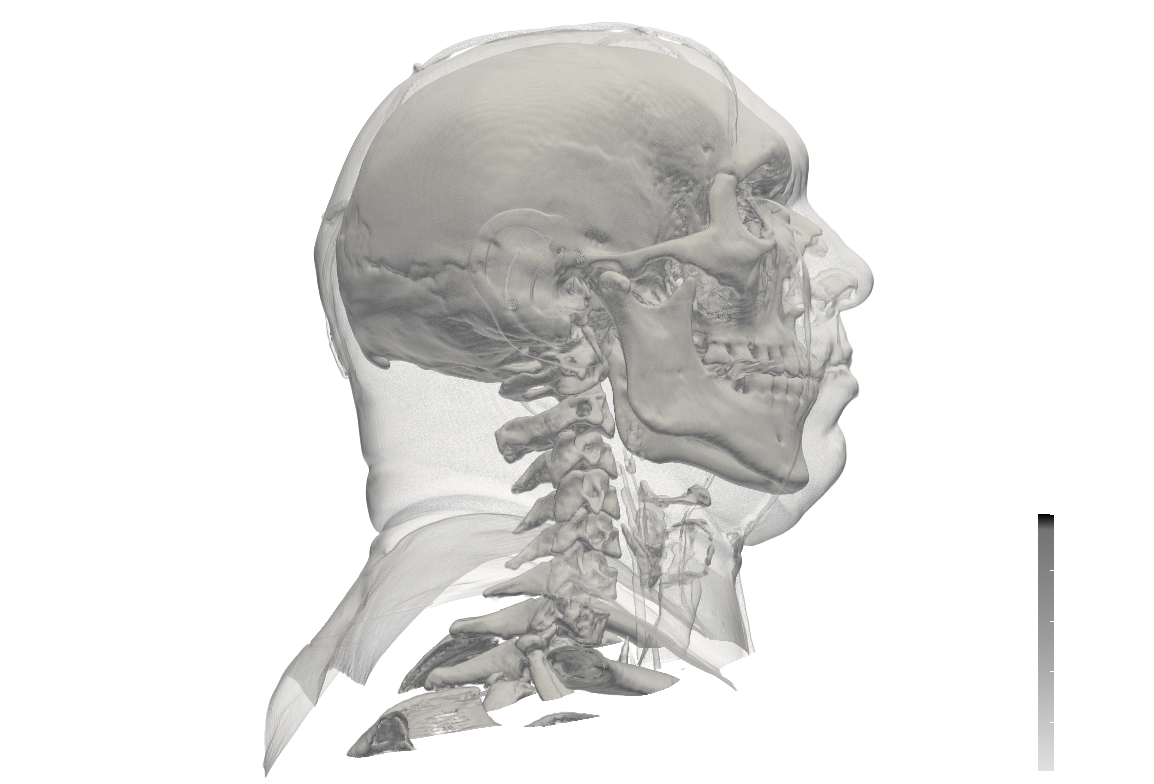
\includegraphics[width=\linewidth]{VisHuman_Head/human_head_1}
  \caption{Resulting visualisation}
\end{subfigure}
\caption{Visualising bones}
\end{figure}

We also tried to expand this concept by using a different color map and a smoother transition to total opacity in order to see which bones have the maximum density. To do so, we used the \textit{Rainbow Uniform} color map. As expected, the most dense bones of the upper part of the body are the teeth.

\begin{figure}[h]
\centering
\begin{subfigure}{.4\textwidth}
  \centering
  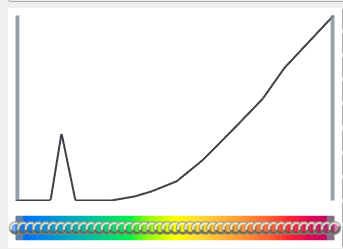
\includegraphics[width=\linewidth]{VisHuman_Head/transfer_function_2}
  \caption{Used transfer function}
\end{subfigure}%
\begin{subfigure}{.6\textwidth}
  \centering
  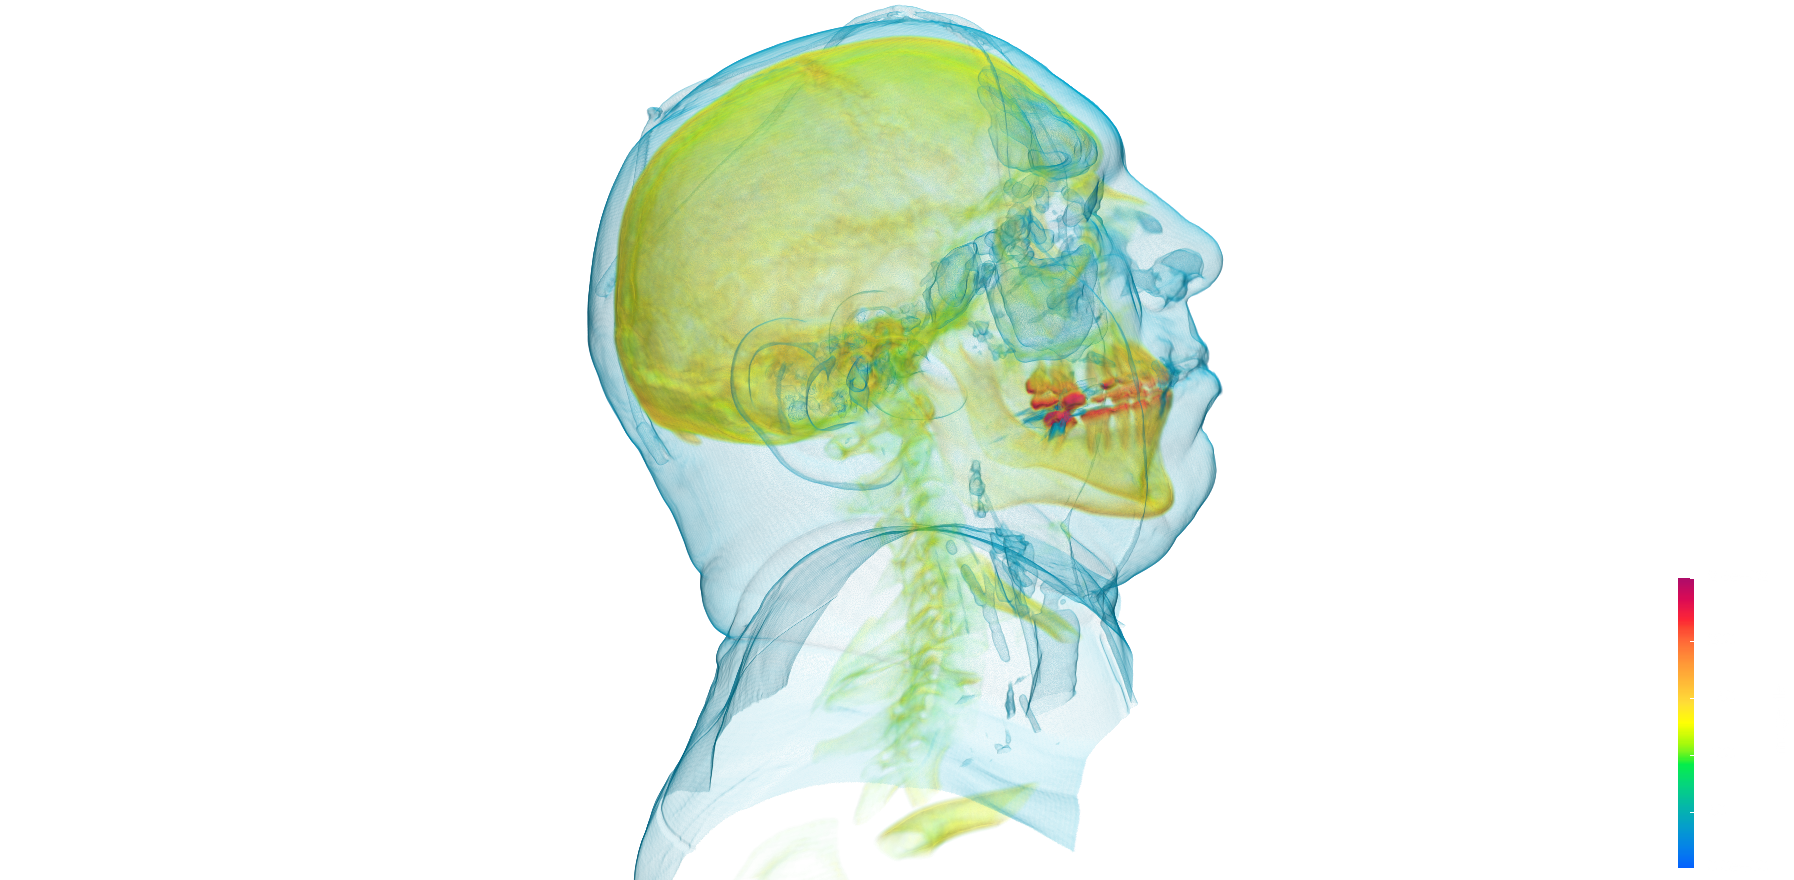
\includegraphics[width=\linewidth]{VisHuman_Head/human_head_2}
  \caption{Resulting visualisation}
\end{subfigure}
\caption{Visualising bones density}
\end{figure}

\subsection {Asian Dragon} 

The Asian Dragon is a \texttt{.ply} file containing a polygonal mesh consisting of 7219045 cells and 3609600 points of \texttt{float} type. The mesh is very dense, so that the surface looks fairly smooth. It requires a lot of zoom in order to see the components of the mesh.

\begin{figure}[h]
\centering
\begin{subfigure}{.5\textwidth}
  \centering
  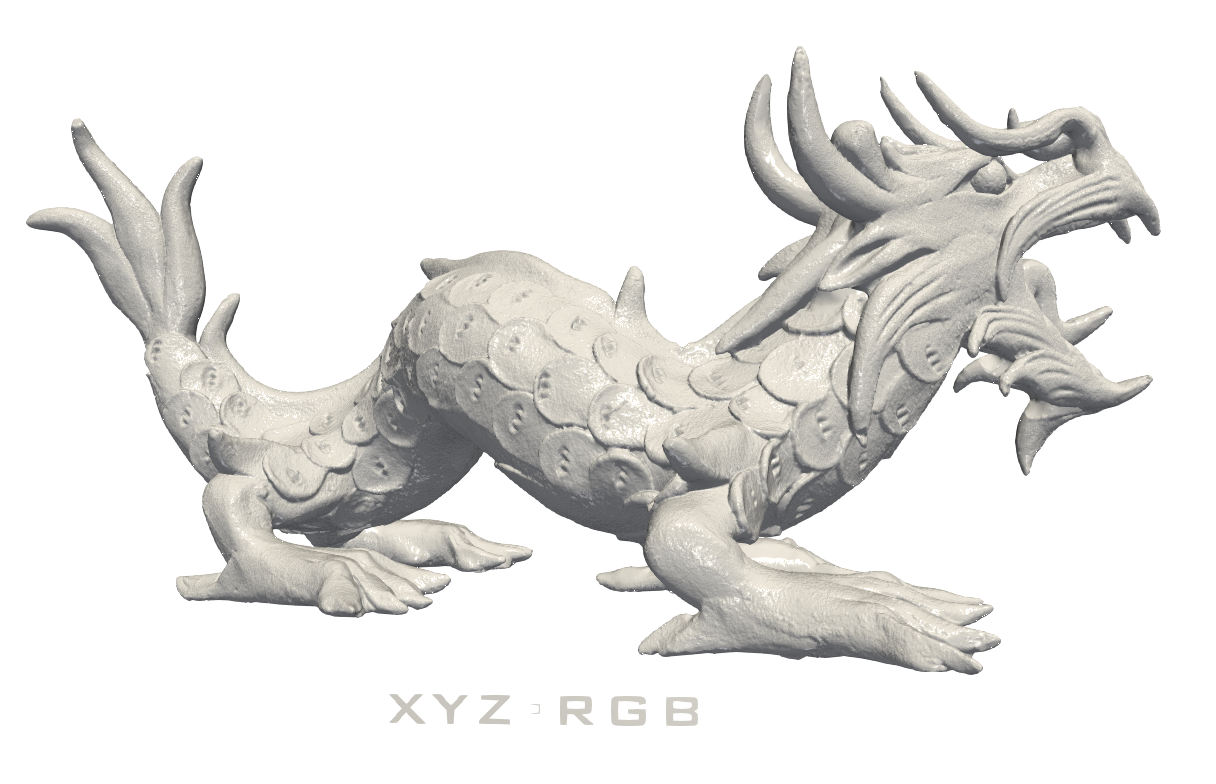
\includegraphics[width=\linewidth]{Asian_Dragon/asian_dragon}
  \caption{Entire dataset, visualised with \textit{surface}  \\
  representation, solid \texttt{\#ffffff} colour and 100\% \\ specular lightning}
\end{subfigure}%
\begin{subfigure}{.5\textwidth}
  \centering
  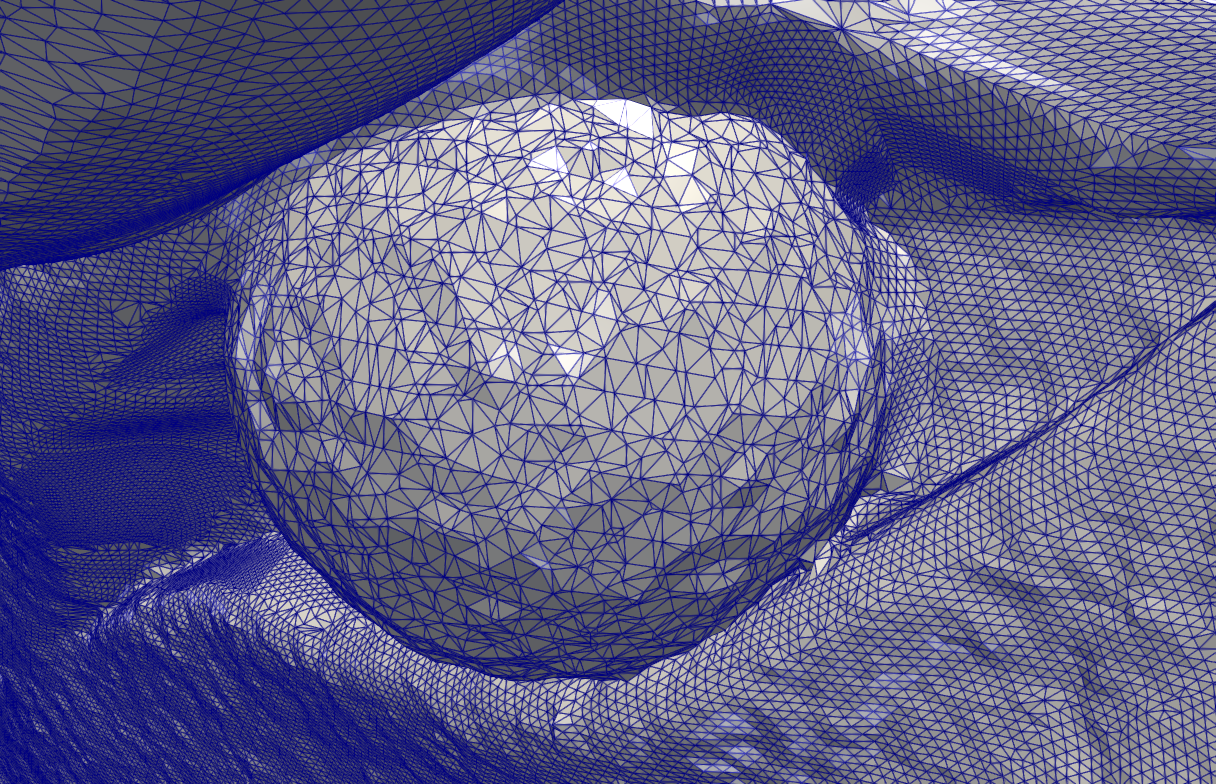
\includegraphics[width=\linewidth]{Asian_Dragon/eye_detail_edges}
  \caption{Eye detail to show the mesh, with \textit{surface with edges} representation, \texttt{\#000080} colour edges}
\end{subfigure}
\caption{Asian Dragon visualisation}
\end{figure}

\newpage
%%%%%%%%%%%%%%%%%%%%%%%%%%%%%%%%%%%%%%%%%%%%
\section {Second part: Tableau}

In the second section we explore the default \textit{Superstore Sales} data set that comes with Tableau.

\subsection {Relation total sales - geographical position}







































\end{document}